\section{Simulated Dataset}

\begin{figure}[h]
    \centering
    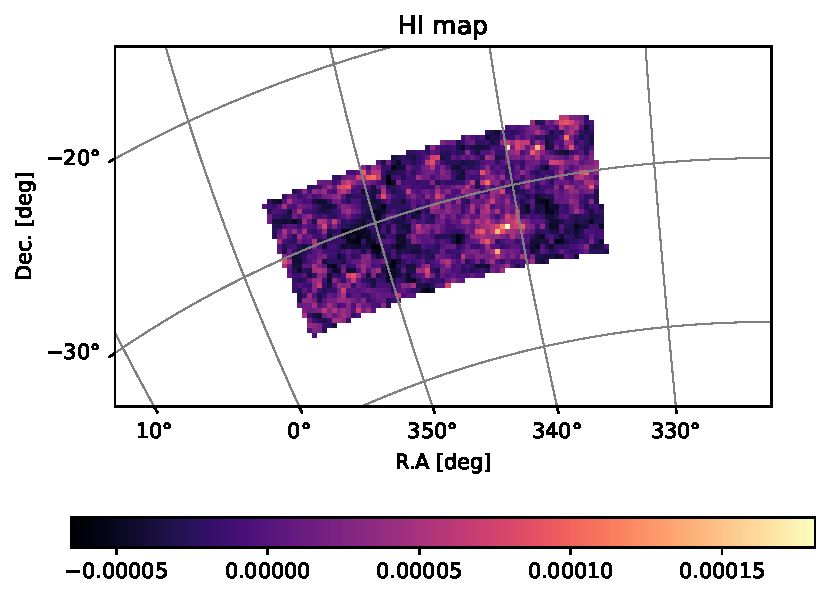
\includegraphics[width=1\linewidth]{outputs/week3/hydrogen_map_wo_foreground.pdf}
    \caption{A cosmological neutral hydrogen (HI) distribution generated from theory without any foregrounds.}
    \label{fig:map_wo_foreground}
\end{figure}

\begin{figure}[h]
    \centering
    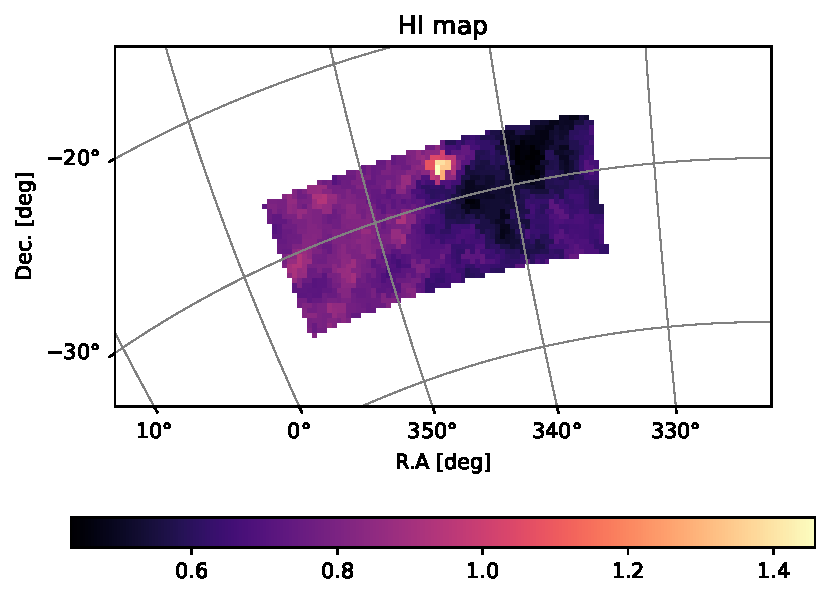
\includegraphics[width=1\linewidth]{outputs/week3/hydrogen_map_w_foreground.pdf}
    \caption{A cosmological neutral hydrogen (HI) distribution generated from theory with foregrounds.}
    \label{fig:map_w_foreground}
\end{figure}

\begin{figure}[h]
    \centering
    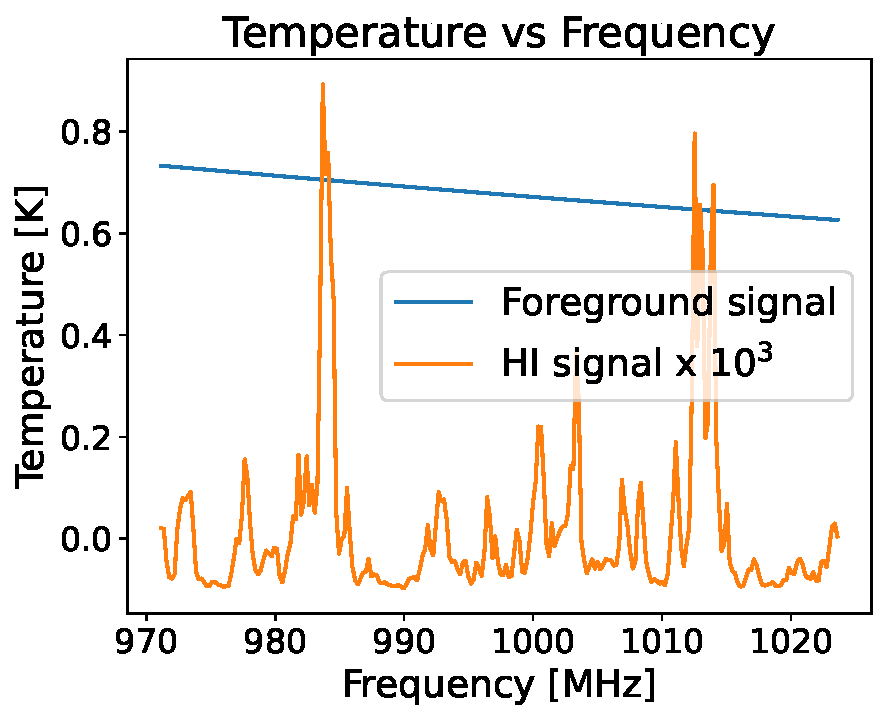
\includegraphics[width=1\linewidth]{outputs/week3/frequency_vs_temperature.pdf}
    \caption{A plot of frequency versus temperature. The foregrounds and HI signal are different in frequency structure. The foregrounds are 4 orders of magnitude larger than the HI signal.}
    \label{fig:frequency_vs_temperature}
\end{figure}

% [1] https://meer21cm.readthedocs.io/en/latest/
A cosmological neutral hydrogen (HI) distribution was generated from theory using the meer21cm package [1] by defining some input model. This gave a survey area and frequency range which gives the cosmological redshifts. These maps generated with just the 21cm signal and the 21cm signal with foreground can be seen in \cref{fig:map_w_foreground} and \cref{fig:map_wo_foreground}. The colour scales for both distributions are different with the foregrounds being four orders of magnitude larger than the 21cm signal. It can also be seen that they are different in frequency structure. It is important to note that this is mock data and not a real observation which would contain telescope beam smoothing, foreground contamination, and thermal noise.

A plot of the frequency versus temperature can be seen in \cref{fig:frequency_vs_temperature}. The foregrounds and HI signal are different in frequency structure. The foregrounds are 4 orders of magnitude larger than the HI signal.

% write more!! maybe
From these HI maps, the power spectrum can be extracted. This power spectrum can be flattened to 1D. See a plot which shows the power spectrum of the data compared to the input data.